
% Default to the notebook output style

    


% Inherit from the specified cell style.




    
\documentclass[11pt]{article}

    \usepackage{wrapfig}
    \usepackage{tikz}
    \usepackage[T1]{fontenc}
    % Nicer default font (+ math font) than Computer Modern for most use cases
    \usepackage{mathpazo}

    % Basic figure setup, for now with no caption control since it's done
    % automatically by Pandoc (which extracts ![](path) syntax from Markdown).
    \usepackage{graphicx}
    % We will generate all images so they have a width \maxwidth. This means
    % that they will get their normal width if they fit onto the page, but
    % are scaled down if they would overflow the margins.
    \makeatletter
    \def\maxwidth{\ifdim\Gin@nat@width>\linewidth\linewidth
    \else\Gin@nat@width\fi}
    \makeatother
    \let\Oldincludegraphics\includegraphics
    % Set max figure width to be 80% of text width, for now hardcoded.
    \renewcommand{\includegraphics}[1]{\Oldincludegraphics[width=.8\maxwidth]{#1}}
    % Ensure that by default, figures have no caption (until we provide a
    % proper Figure object with a Caption API and a way to capture that
    % in the conversion process - todo).
    \usepackage{caption}
    \DeclareCaptionLabelFormat{nolabel}{}
    \captionsetup{labelformat=nolabel}

    \usepackage{adjustbox} % Used to constrain images to a maximum size 
    \usepackage{xcolor} % Allow colors to be defined
    \usepackage{enumerate} % Needed for markdown enumerations to work
    \usepackage{geometry} % Used to adjust the document margins
    \usepackage{amsmath} % Equations
    \usepackage{amssymb} % Equations
    \usepackage{textcomp} % defines textquotesingle
    % Hack from http://tex.stackexchange.com/a/47451/13684:
    \AtBeginDocument{%
        \def\PYZsq{\textquotesingle}% Upright quotes in Pygmentized code
    }
    \usepackage{upquote} % Upright quotes for verbatim code
    \usepackage{eurosym} % defines \euro
    \usepackage[mathletters]{ucs} % Extended unicode (utf-8) support
    \usepackage[utf8x]{inputenc} % Allow utf-8 characters in the tex document
    \usepackage{fancyvrb} % verbatim replacement that allows latex
    \usepackage{grffile} % extends the file name processing of package graphics 
                         % to support a larger range 
    % The hyperref package gives us a pdf with properly built
    % internal navigation ('pdf bookmarks' for the table of contents,
    % internal cross-reference links, web links for URLs, etc.)
    \usepackage{hyperref}
    \usepackage{longtable} % longtable support required by pandoc >1.10
    \usepackage{booktabs}  % table support for pandoc > 1.12.2
    \usepackage[inline]{enumitem} % IRkernel/repr support (it uses the enumerate* environment)
    \usepackage[normalem]{ulem} % ulem is needed to support strikethroughs (\sout)
                                % normalem makes italics be italics, not underlines
    

    
    
    % Colors for the hyperref package
    \definecolor{urlcolor}{rgb}{0,.145,.698}
    \definecolor{linkcolor}{rgb}{.71,0.21,0.01}
    \definecolor{citecolor}{rgb}{.12,.54,.11}

    % ANSI colors
    \definecolor{ansi-black}{HTML}{3E424D}
    \definecolor{ansi-black-intense}{HTML}{282C36}
    \definecolor{ansi-red}{HTML}{E75C58}
    \definecolor{ansi-red-intense}{HTML}{B22B31}
    \definecolor{ansi-green}{HTML}{00A250}
    \definecolor{ansi-green-intense}{HTML}{007427}
    \definecolor{ansi-yellow}{HTML}{DDB62B}
    \definecolor{ansi-yellow-intense}{HTML}{B27D12}
    \definecolor{ansi-blue}{HTML}{208FFB}
    \definecolor{ansi-blue-intense}{HTML}{0065CA}
    \definecolor{ansi-magenta}{HTML}{D160C4}
    \definecolor{ansi-magenta-intense}{HTML}{A03196}
    \definecolor{ansi-cyan}{HTML}{60C6C8}
    \definecolor{ansi-cyan-intense}{HTML}{258F8F}
    \definecolor{ansi-white}{HTML}{C5C1B4}
    \definecolor{ansi-white-intense}{HTML}{A1A6B2}

    % commands and environments needed by pandoc snippets
    % extracted from the output of `pandoc -s`
    \providecommand{\tightlist}{%
      \setlength{\itemsep}{0pt}\setlength{\parskip}{0pt}}
    \DefineVerbatimEnvironment{Highlighting}{Verbatim}{commandchars=\\\{\}}
    % Add ',fontsize=\small' for more characters per line
    \newenvironment{Shaded}{}{}
    \newcommand{\KeywordTok}[1]{\textcolor[rgb]{0.00,0.44,0.13}{\textbf{{#1}}}}
    \newcommand{\DataTypeTok}[1]{\textcolor[rgb]{0.56,0.13,0.00}{{#1}}}
    \newcommand{\DecValTok}[1]{\textcolor[rgb]{0.25,0.63,0.44}{{#1}}}
    \newcommand{\BaseNTok}[1]{\textcolor[rgb]{0.25,0.63,0.44}{{#1}}}
    \newcommand{\FloatTok}[1]{\textcolor[rgb]{0.25,0.63,0.44}{{#1}}}
    \newcommand{\CharTok}[1]{\textcolor[rgb]{0.25,0.44,0.63}{{#1}}}
    \newcommand{\StringTok}[1]{\textcolor[rgb]{0.25,0.44,0.63}{{#1}}}
    \newcommand{\CommentTok}[1]{\textcolor[rgb]{0.38,0.63,0.69}{\textit{{#1}}}}
    \newcommand{\OtherTok}[1]{\textcolor[rgb]{0.00,0.44,0.13}{{#1}}}
    \newcommand{\AlertTok}[1]{\textcolor[rgb]{1.00,0.00,0.00}{\textbf{{#1}}}}
    \newcommand{\FunctionTok}[1]{\textcolor[rgb]{0.02,0.16,0.49}{{#1}}}
    \newcommand{\RegionMarkerTok}[1]{{#1}}
    \newcommand{\ErrorTok}[1]{\textcolor[rgb]{1.00,0.00,0.00}{\textbf{{#1}}}}
    \newcommand{\NormalTok}[1]{{#1}}
    
    % Additional commands for more recent versions of Pandoc
    \newcommand{\ConstantTok}[1]{\textcolor[rgb]{0.53,0.00,0.00}{{#1}}}
    \newcommand{\SpecialCharTok}[1]{\textcolor[rgb]{0.25,0.44,0.63}{{#1}}}
    \newcommand{\VerbatimStringTok}[1]{\textcolor[rgb]{0.25,0.44,0.63}{{#1}}}
    \newcommand{\SpecialStringTok}[1]{\textcolor[rgb]{0.73,0.40,0.53}{{#1}}}
    \newcommand{\ImportTok}[1]{{#1}}
    \newcommand{\DocumentationTok}[1]{\textcolor[rgb]{0.73,0.13,0.13}{\textit{{#1}}}}
    \newcommand{\AnnotationTok}[1]{\textcolor[rgb]{0.38,0.63,0.69}{\textbf{\textit{{#1}}}}}
    \newcommand{\CommentVarTok}[1]{\textcolor[rgb]{0.38,0.63,0.69}{\textbf{\textit{{#1}}}}}
    \newcommand{\VariableTok}[1]{\textcolor[rgb]{0.10,0.09,0.49}{{#1}}}
    \newcommand{\ControlFlowTok}[1]{\textcolor[rgb]{0.00,0.44,0.13}{\textbf{{#1}}}}
    \newcommand{\OperatorTok}[1]{\textcolor[rgb]{0.40,0.40,0.40}{{#1}}}
    \newcommand{\BuiltInTok}[1]{{#1}}
    \newcommand{\ExtensionTok}[1]{{#1}}
    \newcommand{\PreprocessorTok}[1]{\textcolor[rgb]{0.74,0.48,0.00}{{#1}}}
    \newcommand{\AttributeTok}[1]{\textcolor[rgb]{0.49,0.56,0.16}{{#1}}}
    \newcommand{\InformationTok}[1]{\textcolor[rgb]{0.38,0.63,0.69}{\textbf{\textit{{#1}}}}}
    \newcommand{\WarningTok}[1]{\textcolor[rgb]{0.38,0.63,0.69}{\textbf{\textit{{#1}}}}}
    
    
    % Define a nice break command that doesn't care if a line doesn't already
    % exist.
    \def\br{\hspace*{\fill} \\* }
    % Math Jax compatability definitions
    \def\gt{>}
    \def\lt{<}
    % Document parameters
    \title{PyNormaliz Tutorial}
    
    
    

    % Pygments definitions
    
\makeatletter
\def\PY@reset{\let\PY@it=\relax \let\PY@bf=\relax%
    \let\PY@ul=\relax \let\PY@tc=\relax%
    \let\PY@bc=\relax \let\PY@ff=\relax}
\def\PY@tok#1{\csname PY@tok@#1\endcsname}
\def\PY@toks#1+{\ifx\relax#1\empty\else%
    \PY@tok{#1}\expandafter\PY@toks\fi}
\def\PY@do#1{\PY@bc{\PY@tc{\PY@ul{%
    \PY@it{\PY@bf{\PY@ff{#1}}}}}}}
\def\PY#1#2{\PY@reset\PY@toks#1+\relax+\PY@do{#2}}

\expandafter\def\csname PY@tok@cs\endcsname{\let\PY@it=\textit\def\PY@tc##1{\textcolor[rgb]{0.25,0.50,0.50}{##1}}}
\expandafter\def\csname PY@tok@kd\endcsname{\let\PY@bf=\textbf\def\PY@tc##1{\textcolor[rgb]{0.00,0.50,0.00}{##1}}}
\expandafter\def\csname PY@tok@ne\endcsname{\let\PY@bf=\textbf\def\PY@tc##1{\textcolor[rgb]{0.82,0.25,0.23}{##1}}}
\expandafter\def\csname PY@tok@si\endcsname{\let\PY@bf=\textbf\def\PY@tc##1{\textcolor[rgb]{0.73,0.40,0.53}{##1}}}
\expandafter\def\csname PY@tok@no\endcsname{\def\PY@tc##1{\textcolor[rgb]{0.53,0.00,0.00}{##1}}}
\expandafter\def\csname PY@tok@cm\endcsname{\let\PY@it=\textit\def\PY@tc##1{\textcolor[rgb]{0.25,0.50,0.50}{##1}}}
\expandafter\def\csname PY@tok@sh\endcsname{\def\PY@tc##1{\textcolor[rgb]{0.73,0.13,0.13}{##1}}}
\expandafter\def\csname PY@tok@mh\endcsname{\def\PY@tc##1{\textcolor[rgb]{0.40,0.40,0.40}{##1}}}
\expandafter\def\csname PY@tok@sx\endcsname{\def\PY@tc##1{\textcolor[rgb]{0.00,0.50,0.00}{##1}}}
\expandafter\def\csname PY@tok@ni\endcsname{\let\PY@bf=\textbf\def\PY@tc##1{\textcolor[rgb]{0.60,0.60,0.60}{##1}}}
\expandafter\def\csname PY@tok@gr\endcsname{\def\PY@tc##1{\textcolor[rgb]{1.00,0.00,0.00}{##1}}}
\expandafter\def\csname PY@tok@ge\endcsname{\let\PY@it=\textit}
\expandafter\def\csname PY@tok@kp\endcsname{\def\PY@tc##1{\textcolor[rgb]{0.00,0.50,0.00}{##1}}}
\expandafter\def\csname PY@tok@se\endcsname{\let\PY@bf=\textbf\def\PY@tc##1{\textcolor[rgb]{0.73,0.40,0.13}{##1}}}
\expandafter\def\csname PY@tok@ch\endcsname{\let\PY@it=\textit\def\PY@tc##1{\textcolor[rgb]{0.25,0.50,0.50}{##1}}}
\expandafter\def\csname PY@tok@bp\endcsname{\def\PY@tc##1{\textcolor[rgb]{0.00,0.50,0.00}{##1}}}
\expandafter\def\csname PY@tok@il\endcsname{\def\PY@tc##1{\textcolor[rgb]{0.40,0.40,0.40}{##1}}}
\expandafter\def\csname PY@tok@kt\endcsname{\def\PY@tc##1{\textcolor[rgb]{0.69,0.00,0.25}{##1}}}
\expandafter\def\csname PY@tok@ow\endcsname{\let\PY@bf=\textbf\def\PY@tc##1{\textcolor[rgb]{0.67,0.13,1.00}{##1}}}
\expandafter\def\csname PY@tok@nd\endcsname{\def\PY@tc##1{\textcolor[rgb]{0.67,0.13,1.00}{##1}}}
\expandafter\def\csname PY@tok@vg\endcsname{\def\PY@tc##1{\textcolor[rgb]{0.10,0.09,0.49}{##1}}}
\expandafter\def\csname PY@tok@m\endcsname{\def\PY@tc##1{\textcolor[rgb]{0.40,0.40,0.40}{##1}}}
\expandafter\def\csname PY@tok@cpf\endcsname{\let\PY@it=\textit\def\PY@tc##1{\textcolor[rgb]{0.25,0.50,0.50}{##1}}}
\expandafter\def\csname PY@tok@gs\endcsname{\let\PY@bf=\textbf}
\expandafter\def\csname PY@tok@vi\endcsname{\def\PY@tc##1{\textcolor[rgb]{0.10,0.09,0.49}{##1}}}
\expandafter\def\csname PY@tok@mb\endcsname{\def\PY@tc##1{\textcolor[rgb]{0.40,0.40,0.40}{##1}}}
\expandafter\def\csname PY@tok@sr\endcsname{\def\PY@tc##1{\textcolor[rgb]{0.73,0.40,0.53}{##1}}}
\expandafter\def\csname PY@tok@fm\endcsname{\def\PY@tc##1{\textcolor[rgb]{0.00,0.00,1.00}{##1}}}
\expandafter\def\csname PY@tok@nl\endcsname{\def\PY@tc##1{\textcolor[rgb]{0.63,0.63,0.00}{##1}}}
\expandafter\def\csname PY@tok@sb\endcsname{\def\PY@tc##1{\textcolor[rgb]{0.73,0.13,0.13}{##1}}}
\expandafter\def\csname PY@tok@sc\endcsname{\def\PY@tc##1{\textcolor[rgb]{0.73,0.13,0.13}{##1}}}
\expandafter\def\csname PY@tok@gp\endcsname{\let\PY@bf=\textbf\def\PY@tc##1{\textcolor[rgb]{0.00,0.00,0.50}{##1}}}
\expandafter\def\csname PY@tok@kn\endcsname{\let\PY@bf=\textbf\def\PY@tc##1{\textcolor[rgb]{0.00,0.50,0.00}{##1}}}
\expandafter\def\csname PY@tok@o\endcsname{\def\PY@tc##1{\textcolor[rgb]{0.40,0.40,0.40}{##1}}}
\expandafter\def\csname PY@tok@gi\endcsname{\def\PY@tc##1{\textcolor[rgb]{0.00,0.63,0.00}{##1}}}
\expandafter\def\csname PY@tok@nn\endcsname{\let\PY@bf=\textbf\def\PY@tc##1{\textcolor[rgb]{0.00,0.00,1.00}{##1}}}
\expandafter\def\csname PY@tok@gh\endcsname{\let\PY@bf=\textbf\def\PY@tc##1{\textcolor[rgb]{0.00,0.00,0.50}{##1}}}
\expandafter\def\csname PY@tok@k\endcsname{\let\PY@bf=\textbf\def\PY@tc##1{\textcolor[rgb]{0.00,0.50,0.00}{##1}}}
\expandafter\def\csname PY@tok@c1\endcsname{\let\PY@it=\textit\def\PY@tc##1{\textcolor[rgb]{0.25,0.50,0.50}{##1}}}
\expandafter\def\csname PY@tok@kc\endcsname{\let\PY@bf=\textbf\def\PY@tc##1{\textcolor[rgb]{0.00,0.50,0.00}{##1}}}
\expandafter\def\csname PY@tok@nt\endcsname{\let\PY@bf=\textbf\def\PY@tc##1{\textcolor[rgb]{0.00,0.50,0.00}{##1}}}
\expandafter\def\csname PY@tok@ss\endcsname{\def\PY@tc##1{\textcolor[rgb]{0.10,0.09,0.49}{##1}}}
\expandafter\def\csname PY@tok@err\endcsname{\def\PY@bc##1{\setlength{\fboxsep}{0pt}\fcolorbox[rgb]{1.00,0.00,0.00}{1,1,1}{\strut ##1}}}
\expandafter\def\csname PY@tok@sd\endcsname{\let\PY@it=\textit\def\PY@tc##1{\textcolor[rgb]{0.73,0.13,0.13}{##1}}}
\expandafter\def\csname PY@tok@mo\endcsname{\def\PY@tc##1{\textcolor[rgb]{0.40,0.40,0.40}{##1}}}
\expandafter\def\csname PY@tok@c\endcsname{\let\PY@it=\textit\def\PY@tc##1{\textcolor[rgb]{0.25,0.50,0.50}{##1}}}
\expandafter\def\csname PY@tok@nv\endcsname{\def\PY@tc##1{\textcolor[rgb]{0.10,0.09,0.49}{##1}}}
\expandafter\def\csname PY@tok@vm\endcsname{\def\PY@tc##1{\textcolor[rgb]{0.10,0.09,0.49}{##1}}}
\expandafter\def\csname PY@tok@mi\endcsname{\def\PY@tc##1{\textcolor[rgb]{0.40,0.40,0.40}{##1}}}
\expandafter\def\csname PY@tok@gu\endcsname{\let\PY@bf=\textbf\def\PY@tc##1{\textcolor[rgb]{0.50,0.00,0.50}{##1}}}
\expandafter\def\csname PY@tok@go\endcsname{\def\PY@tc##1{\textcolor[rgb]{0.53,0.53,0.53}{##1}}}
\expandafter\def\csname PY@tok@s1\endcsname{\def\PY@tc##1{\textcolor[rgb]{0.73,0.13,0.13}{##1}}}
\expandafter\def\csname PY@tok@mf\endcsname{\def\PY@tc##1{\textcolor[rgb]{0.40,0.40,0.40}{##1}}}
\expandafter\def\csname PY@tok@w\endcsname{\def\PY@tc##1{\textcolor[rgb]{0.73,0.73,0.73}{##1}}}
\expandafter\def\csname PY@tok@gt\endcsname{\def\PY@tc##1{\textcolor[rgb]{0.00,0.27,0.87}{##1}}}
\expandafter\def\csname PY@tok@vc\endcsname{\def\PY@tc##1{\textcolor[rgb]{0.10,0.09,0.49}{##1}}}
\expandafter\def\csname PY@tok@cp\endcsname{\def\PY@tc##1{\textcolor[rgb]{0.74,0.48,0.00}{##1}}}
\expandafter\def\csname PY@tok@s\endcsname{\def\PY@tc##1{\textcolor[rgb]{0.73,0.13,0.13}{##1}}}
\expandafter\def\csname PY@tok@sa\endcsname{\def\PY@tc##1{\textcolor[rgb]{0.73,0.13,0.13}{##1}}}
\expandafter\def\csname PY@tok@gd\endcsname{\def\PY@tc##1{\textcolor[rgb]{0.63,0.00,0.00}{##1}}}
\expandafter\def\csname PY@tok@s2\endcsname{\def\PY@tc##1{\textcolor[rgb]{0.73,0.13,0.13}{##1}}}
\expandafter\def\csname PY@tok@nc\endcsname{\let\PY@bf=\textbf\def\PY@tc##1{\textcolor[rgb]{0.00,0.00,1.00}{##1}}}
\expandafter\def\csname PY@tok@nb\endcsname{\def\PY@tc##1{\textcolor[rgb]{0.00,0.50,0.00}{##1}}}
\expandafter\def\csname PY@tok@dl\endcsname{\def\PY@tc##1{\textcolor[rgb]{0.73,0.13,0.13}{##1}}}
\expandafter\def\csname PY@tok@na\endcsname{\def\PY@tc##1{\textcolor[rgb]{0.49,0.56,0.16}{##1}}}
\expandafter\def\csname PY@tok@nf\endcsname{\def\PY@tc##1{\textcolor[rgb]{0.00,0.00,1.00}{##1}}}
\expandafter\def\csname PY@tok@kr\endcsname{\let\PY@bf=\textbf\def\PY@tc##1{\textcolor[rgb]{0.00,0.50,0.00}{##1}}}

\def\PYZbs{\char`\\}
\def\PYZus{\char`\_}
\def\PYZob{\char`\{}
\def\PYZcb{\char`\}}
\def\PYZca{\char`\^}
\def\PYZam{\char`\&}
\def\PYZlt{\char`\<}
\def\PYZgt{\char`\>}
\def\PYZsh{\char`\#}
\def\PYZpc{\char`\%}
\def\PYZdl{\char`\$}
\def\PYZhy{\char`\-}
\def\PYZsq{\char`\'}
\def\PYZdq{\char`\"}
\def\PYZti{\char`\~}
% for compatibility with earlier versions
\def\PYZat{@}
\def\PYZlb{[}
\def\PYZrb{]}
\makeatother


    % Exact colors from NB
    \definecolor{incolor}{rgb}{0.0, 0.0, 0.5}
    \definecolor{outcolor}{rgb}{0.545, 0.0, 0.0}



    
    % Prevent overflowing lines due to hard-to-break entities
    \sloppy 
    % Setup hyperref package
    \hypersetup{
      breaklinks=true,  % so long urls are correctly broken across lines
      colorlinks=true,
      urlcolor=urlcolor,
      linkcolor=linkcolor,
      citecolor=citecolor,
      }
    % Slightly bigger margins than the latex defaults
    
    \geometry{verbose,tmargin=1in,bmargin=1in,lmargin=1in,rmargin=1in}
    
    \date{}
    \author{Winfried Bruns, Sebastian Gutsche, Justin Shenk, Richard Sieg}

    \begin{document}
    
    
    \maketitle
    
    

    
 
This small tutorial introduces the main syntax of the Python interface
PyNormaliz for Normaliz.

To install PyNormaliz on your machine, download PyNormaliz and run
\begin{Verbatim}
python setup.py install
\end{Verbatim}
or
\begin{Verbatim}
pip install .
\end{Verbatim}

If you are using python3 you might need to enter python3/pip3 instead of
python/pip.

    \section{A cone in dimension 2}\label{example-1-a-cone-in-dimension-2}

\begin{wrapfigure}[4]{R}{0.2\textwidth}
	\vspace{-0.2cm}
	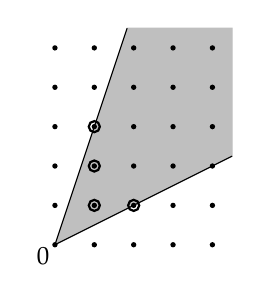
\begin{tikzpicture}[scale=0.5]
	\filldraw[lightgray] (0,0) -- (1.833,5.5) -- (4.5,5.5) -- (4.5,2.25) -- cycle;
	\draw (0,0) -- (1.833,5.5);
	\draw (0,0) -- (4.5,2.25) node at (-0.3,-0.3){\small $0$};
	\foreach \x in {0,...,4}
	\foreach \y in {0,...,5}
	{
		\filldraw[fill=black] (\x,\y)  circle (1.5pt);
	}
	\draw[black,thick] (1,1) circle (4pt);
	\draw[black,thick] (1,2) circle (4pt);
	\draw[black,thick] (1,3) circle (4pt);
	\draw[black,thick] (2,1) circle (4pt);
	\end{tikzpicture}	
\end{wrapfigure}

 We want to investigate the cone
\(C=\mathbb{R}_{+}(2,1)+\mathbb{R}_{+}(1,3)\subset\mathbb{R}^2\).



In the cone constructor of PyNormaliz, we specify the input type
("cone") and an input matrix for this input type.

To compute its Hilbert basis we use the point operator and call
HilbertBasis() on our cone.

    \begin{Verbatim}[commandchars=\\\{\}]
{\color{incolor}In [{\color{incolor}1}]:} \PY{k+kn}{from} \PY{n+nn}{PyNormaliz} \PY{k}{import} \PY{o}{*} \PY{c+c1}{\PYZsh{} or import PyNormaliz}
        
        \PY{n}{gen} \PY{o}{=} \PY{p}{[}\PY{p}{[}\PY{l+m+mi}{1}\PY{p}{,}\PY{l+m+mi}{3}\PY{p}{]}\PY{p}{,}\PY{p}{[}\PY{l+m+mi}{2}\PY{p}{,}\PY{l+m+mi}{1}\PY{p}{]}\PY{p}{]}
        \PY{n}{C} \PY{o}{=} \PY{n}{Cone}\PY{p}{(}\PY{n}{cone}\PY{o}{=}\PY{n}{gen}\PY{p}{)}
        \PY{n}{C}\PY{o}{.}\PY{n}{HilbertBasis}\PY{p}{(}\PY{p}{)}
\end{Verbatim}

            \begin{Verbatim}[commandchars=\\\{\}]
{\color{outcolor}Out[{\color{outcolor}1}]:} [[1, 1], [1, 2], [1, 3], [2, 1]]
\end{Verbatim}
        
    We can also use inequalities as an input. We also check that the extreme
rays of the new cone are really the generators of the previous one.

    \begin{Verbatim}[commandchars=\\\{\}]
{\color{incolor}In [{\color{incolor}2}]:} \PY{n}{ineq} \PY{o}{=} \PY{p}{[}\PY{p}{[}\PY{o}{\PYZhy{}}\PY{l+m+mi}{1}\PY{p}{,}\PY{l+m+mi}{2}\PY{p}{]}\PY{p}{,}\PY{p}{[}\PY{l+m+mi}{3}\PY{p}{,}\PY{o}{\PYZhy{}}\PY{l+m+mi}{1}\PY{p}{]}\PY{p}{]}
        \PY{n}{C2} \PY{o}{=} \PY{n}{Cone}\PY{p}{(}\PY{n}{inequalities}\PY{o}{=}\PY{n}{ineq}\PY{p}{)}
        \PY{n}{gen2} \PY{o}{=} \PY{n}{cone2}\PY{o}{.}\PY{n}{ExtremeRays}\PY{p}{(}\PY{p}{)}
        \PY{n+nb}{print}\PY{p}{(}\PY{n}{gen}\PY{o}{==}\PY{n}{gen2}\PY{p}{)}
        \PY{n}{HB2} \PY{o}{=} \PY{n}{C2}\PY{o}{.}\PY{n}{HilbertBasis}\PY{p}{(}\PY{p}{)}
        \PY{n+nb}{print}\PY{p}{(}\PY{n}{HB2}\PY{p}{)}
\end{Verbatim}

    \begin{Verbatim}[commandchars=\\\{\}]
True
[[1, 1], [1, 2], [1, 3], [2, 1]]

    \end{Verbatim}

    \section{A lattice
polytope}\label{example-2-a-lattice-polytope}

\begin{wrapfigure}[4]{R}{0.2\textwidth}
	\vspace{-0.2cm}
\tikzset{facet style/.style={opacity=1.0,very thick,line,join=round}}
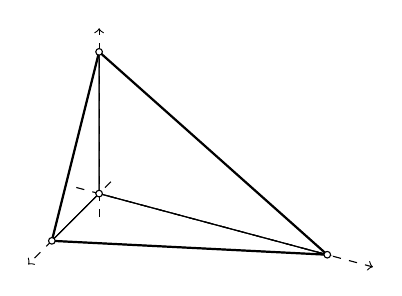
\begin{tikzpicture}[x  = {(-0.5cm,-0.5cm)},
y  = {(0.9659cm,-0.25882cm)},
z  = {(0cm,1cm)},
scale = 0.6]
\draw [->,dashed] (-0.5, 0, 0) -- (3.0,0,0);

\draw [->,dashed] (0, -0.5, 0) -- (0,6.0,0);

\draw [->,dashed] (0, 0, -0.5) -- (0,0,3.5);

\draw[thin] (0,0,0) -- (2,0,0) -- (0,5,0) -- cycle;
\draw[thin] (0,0,0) -- (2,0,0) -- (0,0,3) -- cycle;
\draw[thin] (0,0,0) -- (0,5,0) -- (0,0,3) -- cycle;
\draw[thick] (2,0,0) -- (0,5,0) -- (0,0,3) -- cycle;

\filldraw[fill=white] (0,0,0) circle (2pt);
\filldraw[fill=white] (2,0,0) circle (2pt);
\filldraw[fill=white] (0,5,0) circle (2pt);
\filldraw[fill=white] (0,0,3) circle (2pt);
\end{tikzpicture}
\end{wrapfigure}

Now we investigate a
lattice simplex, which is not normal/integrally closed.

The inpute type is "polytope". Note that we do not need a homogenizing
variable but really specify the points in their actual dimension.

We compute its Hilbert series and Ehrhart polynomial, which are:

Hilbert series: \(H(t)=\frac{1+14t+15t^2}{(1-t)^4}\)

Ehrhart polynomial: \(p(k)=1+4k+8k^2+5k^3\)

    \begin{Verbatim}[commandchars=\\\{\}]
{\color{incolor}In [{\color{incolor}3}]:} \PY{n}{vertices} \PY{o}{=} \PY{p}{[}\PY{p}{[}\PY{l+m+mi}{0}\PY{p}{,}\PY{l+m+mi}{0}\PY{p}{,}\PY{l+m+mi}{0}\PY{p}{]}\PY{p}{,}\PY{p}{[}\PY{l+m+mi}{2}\PY{p}{,}\PY{l+m+mi}{0}\PY{p}{,}\PY{l+m+mi}{0}\PY{p}{]}\PY{p}{,}\PY{p}{[}\PY{l+m+mi}{0}\PY{p}{,}\PY{l+m+mi}{3}\PY{p}{,}\PY{l+m+mi}{0}\PY{p}{]}\PY{p}{,}\PY{p}{[}\PY{l+m+mi}{0}\PY{p}{,}\PY{l+m+mi}{0}\PY{p}{,}\PY{l+m+mi}{5}\PY{p}{]}\PY{p}{]}
        \PY{n}{poly} \PY{o}{=} \PY{n}{Cone}\PY{p}{(}\PY{n}{polytope}\PY{o}{=}\PY{n}{vertices}\PY{p}{)}
        \PY{n}{HB} \PY{o}{=} \PY{n}{poly}\PY{o}{.}\PY{n}{HilbertBasis}\PY{p}{(}\PY{p}{)}
        \PY{n+nb}{print}\PY{p}{(}\PY{n+nb}{len}\PY{p}{(}\PY{n}{HB}\PY{p}{)}\PY{p}{)}
        \PY{n+nb}{print}\PY{p}{(}\PY{n}{poly}\PY{o}{.}\PY{n}{IsDeg1HilbertBasis}\PY{p}{(}\PY{p}{)}\PY{p}{)}
        \PY{n+nb}{print}\PY{p}{(}\PY{n}{poly}\PY{o}{.}\PY{n}{HilbertSeries}\PY{p}{(}\PY{p}{)}\PY{p}{)} 
        \PY{n+nb}{print}\PY{p}{(}\PY{n}{poly}\PY{o}{.}\PY{n}{HilbertQuasiPolynomial}\PY{p}{(}\PY{p}{)}\PY{p}{)}
\end{Verbatim}

    \begin{Verbatim}[commandchars=\\\{\}]
19
False
[[1, 14, 15], [1, 1, 1, 1], 0]
[[1, 4, 8, 5], 1]

    \end{Verbatim}

    If we are only interested in the lattic points, we compute them via the
command Deg1Elements. Note that the output now has the homogenizing
variable as last coordinate.

    \begin{Verbatim}[commandchars=\\\{\}]
{\color{incolor}In [{\color{incolor}4}]:} \PY{n}{LP} \PY{o}{=} \PY{n}{poly}\PY{o}{.}\PY{n}{Deg1Elements}\PY{p}{(}\PY{p}{)}
        \PY{n+nb}{print}\PY{p}{(}\PY{n+nb}{len}\PY{p}{(}\PY{n}{LP}\PY{p}{)}\PY{p}{)}
        \PY{n+nb}{print}\PY{p}{(}\PY{n}{LP}\PY{p}{)}
\end{Verbatim}

    \begin{Verbatim}[commandchars=\\\{\}]
18
[[0, 0, 0, 1], [0, 0, 1, 1], [0, 0, 2, 1], [0, 0, 3, 1], [0, 0, 4, 1], [0, 0, 5, 1], 
[0, 1, 0, 1], [0, 1, 1, 1], [0, 1, 2, 1], [0, 1, 3, 1], [0, 2, 0, 1], [0, 2, 1, 1], 
[0, 3, 0, 1], [1, 0, 0, 1], [1, 0, 1, 1], [1, 0, 2, 1], [1, 1, 0, 1], [2, 0, 0, 1]]

    \end{Verbatim}

    If you would like to have a list of all already computed properties and
data, you can use the
\begin{Verbatim}
print_properties()
\end{Verbatim}
function.

    \begin{Verbatim}[commandchars=\\\{\}]
{\color{incolor}In [{\color{incolor}12}]:} \PY{n}{poly}\PY{o}{.}\PY{n}{print\PYZus{}properties}\PY{p}{(}\PY{p}{)}
\end{Verbatim}

    \begin{Verbatim}[commandchars=\\\{\}]
Generators:
[[0, 0, 0, 1], [0, 0, 5, 1], [0, 3, 0, 1], [2, 0, 0, 1]]


ExtremeRays:
[[0, 0, 0, 1], [0, 0, 5, 1], [0, 3, 0, 1], [2, 0, 0, 1]]


SupportHyperplanes:
[[-15, -10, -6, 30], [0, 0, 1, 0], [0, 1, 0, 0], [1, 0, 0, 0]]

...
    \end{Verbatim}

    \section{A rational
polytope}\label{example-3-a-rational-polytope}

\begin{wrapfigure}[4]{R}{0.2\textwidth}
	\vspace{-0.2cm}
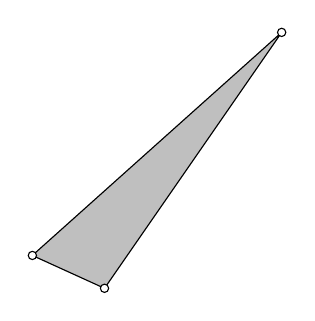
\begin{tikzpicture}[scale=1.0]
\filldraw[lightgray] (2.5,1.5) -- (-0.666,-1.333) -- (0.25,-1.75) -- cycle;	
\draw (2.5,1.5) -- (-0.666,-1.333) -- (0.25,-1.75) -- cycle;	
\filldraw[fill=white] (2.5,1.5)circle (1.5pt);
\filldraw[fill=white] (-0.666,-1.333) circle (1.5pt);
\filldraw[fill=white] (0.25,-1.75) circle (1.5pt);
\end{tikzpicture}
\end{wrapfigure}

We construct a polytope with vertices
\((5/2,3/2),(-2/3,-4/3),(1/4,-7/4)\).

This is the first time we enter two different and compatible input types
into the constructor. With the grading we declare the last coordinate to
be the denominator of the vertices.

    \begin{Verbatim}[commandchars=\\\{\}]
{\color{incolor}In [{\color{incolor}5}]:} \PY{n}{rat\PYZus{}vert} \PY{o}{=} \PY{p}{[}\PY{p}{[}\PY{l+m+mi}{5}\PY{p}{,}\PY{l+m+mi}{3}\PY{p}{,}\PY{l+m+mi}{2}\PY{p}{]}\PY{p}{,}\PY{p}{[}\PY{o}{\PYZhy{}}\PY{l+m+mi}{2}\PY{p}{,}\PY{o}{\PYZhy{}}\PY{l+m+mi}{4}\PY{p}{,}\PY{l+m+mi}{3}\PY{p}{]}\PY{p}{,}\PY{p}{[}\PY{l+m+mi}{1}\PY{p}{,}\PY{o}{\PYZhy{}}\PY{l+m+mi}{7}\PY{p}{,}\PY{l+m+mi}{4}\PY{p}{]}\PY{p}{]}
        \PY{n}{g} \PY{o}{=} \PY{p}{[}\PY{l+m+mi}{0}\PY{p}{,}\PY{l+m+mi}{0}\PY{p}{,}\PY{l+m+mi}{1}\PY{p}{]}
        \PY{n}{rat\PYZus{}poly} \PY{o}{=} \PY{n}{Cone}\PY{p}{(}\PY{n}{cone}\PY{o}{=}\PY{n}{rat\PYZus{}vert}\PY{p}{,}\PY{n}{grading}\PY{o}{=}\PY{n}{g}\PY{p}{)}
        \PY{n+nb}{print}\PY{p}{(}\PY{n}{rat\PYZus{}poly}\PY{o}{.}\PY{n}{HilbertSeries}\PY{p}{(}\PY{p}{)}\PY{p}{)}
        \PY{n+nb}{print}\PY{p}{(}\PY{n}{rat\PYZus{}poly}\PY{o}{.}\PY{n}{HilbertQuasiPolynomial}\PY{p}{(}\PY{p}{)}\PY{p}{)}
\end{Verbatim}

    \begin{Verbatim}[commandchars=\\\{\}]
[[1, 1, 4, 4, 5, 2, 4, 6, 3, 2, 6, 4, 2, 3], [1, 1, 12], 0]
[[24, 6, 47], [19, 6, 47], [16, 6, 47], [15, 6, 47], [40, 6, 47], 
[19, 6, 47], [0, 6, 47], [31, 6, 47], [40, 6, 47], [3, 6, 47], 
[16, 6, 47], [31, 6, 47], 24]

    \end{Verbatim}

\begin{wrapfigure}[4]{R}{0.2\textwidth}
	\vspace{-0.2cm}
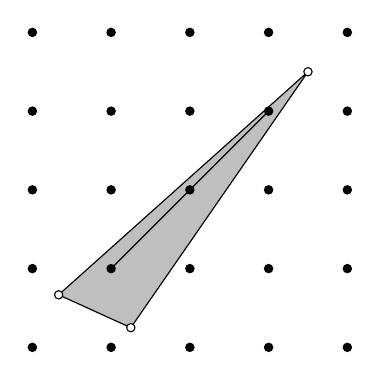
\begin{tikzpicture}[scale=1.0]

\filldraw[lightgray] (2.5,1.5) -- (-0.666,-1.333) -- (0.25,-1.75) -- cycle;	
\draw (2.5,1.5) -- (-0.666,-1.333) -- (0.25,-1.75) -- cycle;	
\filldraw[fill=white] (2.5,1.5)circle (1.5pt);
\filldraw[fill=white] (-0.666,-1.333) circle (1.5pt);
\filldraw[fill=white] (0.25,-1.75) circle (1.5pt);
\foreach \x in {-1,...,3}
\foreach \y in {-2,...,2}
{
	\filldraw[fill=black] (\x,\y)  circle (1.5pt);
}
\draw (0,-1) -- (2,1);
\end{tikzpicture}
\end{wrapfigure}

 We compute the integer
hull of this polytope which is again a cone object and thus we can
access its vertices or support hyperplanes.

    \begin{Verbatim}[commandchars=\\\{\}]
{\color{incolor}In [{\color{incolor}13}]:} \PY{n}{int\PYZus{}hull} \PY{o}{=} \PY{n}{rat\PYZus{}poly}\PY{o}{.}\PY{n}{IntegerHull}\PY{p}{(}\PY{p}{)}
         \PY{n+nb}{print}\PY{p}{(}\PY{n}{int\PYZus{}hull}\PY{o}{.}\PY{n}{VerticesOfPolyhedron}\PY{p}{(}\PY{p}{)}\PY{p}{)}
         \PY{n+nb}{print}\PY{p}{(}\PY{n}{int\PYZus{}hull}\PY{o}{.}\PY{n}{SupportHyperplanes}\PY{p}{(}\PY{p}{)}\PY{p}{)}
         \PY{n+nb}{print}\PY{p}{(}\PY{n}{int\PYZus{}hull}\PY{o}{.}\PY{n}{Equations}\PY{p}{(}\PY{p}{)}\PY{p}{)}
    \end{Verbatim}
    
    \begin{Verbatim}[commandchars=\\\{\}]
    [[0, -1, 1], [2, 1, 1]]
    [[1, -2, 0], [1, 0, 0]]
    [[1, -1, -1]]
    
    \end{Verbatim}

    \section{A polyhedron}\label{example-4-a-polyhedron}

\begin{wrapfigure}[7]{R}{0.2\textwidth}
	\vspace{-0.2cm}
	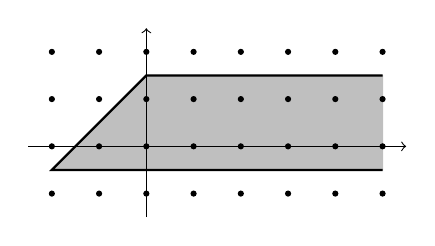
\begin{tikzpicture}[scale=0.6]
	
	\filldraw[lightgray] (5,-0.5) -- (-2,-0.5) -- (0,1.5) -- (5,1.5) -- cycle;
	
	\foreach \x in {-2,...,5}
	\foreach \y in {-1,...,2}
	{
		\filldraw[fill=black] (\x,\y)  circle (1.5pt);
	}
	\draw[->] (-2.5,0) -- (5.5,0);
	\draw[->] (0,-1.5) -- (0,2.5);
	\draw[thick] (5,-0.5) -- (-2,-0.5) -- (0,1.5) -- (5,1.5); 
	\end{tikzpicture}
\end{wrapfigure}

We define a polyhedron by inequalties: 

\begin{align*}
2x_2&\geq -1 \\
2x_2 &\leq 3 \\
-2x_1+2x_2&\leq 3 
\end{align*}

The input type is "inhom\_inequalities" where a row
\((a_1,\ldots,a_n,b)\) in the input matrix defines the inequality

\begin{equation*}a_1x_1 +\dots+a_nx_n+b\geq0.\end{equation*}

In this case, HilbertBasis() returns the Hilbert basis of the recession
cone associated to the polyhedron.

    \begin{Verbatim}[commandchars=\\\{\}]
{\color{incolor}In [{\color{incolor}7}]:} \PY{n}{ineq2} \PY{o}{=} \PY{p}{[}\PY{p}{[}\PY{l+m+mi}{0}\PY{p}{,}\PY{l+m+mi}{2}\PY{p}{,}\PY{l+m+mi}{1}\PY{p}{]}\PY{p}{,}\PY{p}{[}\PY{l+m+mi}{0}\PY{p}{,}\PY{o}{\PYZhy{}}\PY{l+m+mi}{2}\PY{p}{,}\PY{l+m+mi}{3}\PY{p}{]}\PY{p}{,}\PY{p}{[}\PY{l+m+mi}{2}\PY{p}{,}\PY{o}{\PYZhy{}}\PY{l+m+mi}{2}\PY{p}{,}\PY{l+m+mi}{3}\PY{p}{]}\PY{p}{]}
        \PY{n}{polyhedron} \PY{o}{=} \PY{n}{Cone}\PY{p}{(}\PY{n}{inhom\PYZus{}inequalities}\PY{o}{=}\PY{n}{ineq2}\PY{p}{)}
        \PY{n}{HB\PYZus{}rec} \PY{o}{=} \PY{n}{polyhedron}\PY{o}{.}\PY{n}{HilbertBasis}\PY{p}{(}\PY{p}{)}
        \PY{n+nb}{print}\PY{p}{(}\PY{n}{HB\PYZus{}rec}\PY{p}{)}
        
        \PY{n}{module\PYZus{}gen} \PY{o}{=} \PY{n}{polyhedron}\PY{o}{.}\PY{n}{ModuleGenerators}\PY{p}{(}\PY{p}{)}
        \PY{n+nb}{print}\PY{p}{(}\PY{n}{module\PYZus{}gen}\PY{p}{)}
        
        \PY{n}{vert\PYZus{}poly} \PY{o}{=} \PY{n}{polyhedron}\PY{o}{.}\PY{n}{VerticesOfPolyhedron}\PY{p}{(}\PY{p}{)}
        \PY{n+nb}{print}\PY{p}{(}\PY{n}{vert\PYZus{}poly}\PY{p}{)}
\end{Verbatim}

    \begin{Verbatim}[commandchars=\\\{\}]
[[1, 0, 0]]
[[-1, 0, 1], [0, 1, 1]]
[[-4, -1, 2], [0, 3, 2]]

    \end{Verbatim}
\begin{wrapfigure}[3]{R}{0.2\textwidth}
	\vspace{-0.2cm}
		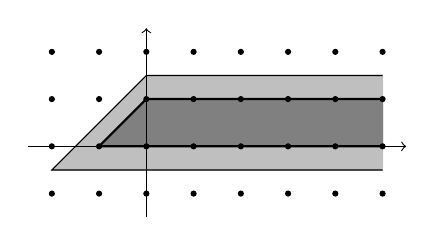
\begin{tikzpicture}[scale=0.6]
		
		\filldraw[lightgray] (5,-0.5) -- (-2,-0.5) -- (0,1.5) -- (5,1.5) -- cycle;
		\filldraw[gray] (5,0) -- (-1,-0) -- (0,1) -- (5,1) -- cycle;
		
		\foreach \x in {-2,...,5}
		\foreach \y in {-1,...,2}
		{
			\filldraw[fill=black] (\x,\y)  circle (1.5pt);
		}
		\draw[->] (-2.5,0) -- (5.5,0);
		\draw[->] (0,-1.5) -- (0,2.5);
		\draw (5,-0.5) -- (-2,-0.5) -- (0,1.5) -- (5,1.5); 
		\draw[thick] (5,0) -- (-1,-0) -- (0,1) -- (5,1);
		\end{tikzpicture}
\end{wrapfigure}


    We can also define the polyhedron via its generators, i.e. its vertices
and generators of its recession cone. 

    \begin{Verbatim}[commandchars=\\\{\}]
{\color{incolor}In [{\color{incolor}8}]:} \PY{n}{poly2} \PY{o}{=} \PY{n}{Cone}\PY{p}{(}\PY{n}{vertices}\PY{o}{=}\PY{n}{vert\PYZus{}poly}\PY{p}{,}\PY{n}{cone}\PY{o}{=}\PY{p}{[}\PY{p}{[}\PY{l+m+mi}{1}\PY{p}{,}\PY{l+m+mi}{0}\PY{p}{]}\PY{p}{]}\PY{p}{)}
        
        \PY{n}{int\PYZus{}hull2} \PY{o}{=} \PY{n}{poly2}\PY{o}{.}\PY{n}{IntegerHull}\PY{p}{(}\PY{p}{)}
        \PY{n+nb}{print}\PY{p}{(}\PY{n}{int\PYZus{}hull2}\PY{o}{.}\PY{n}{VerticesOfPolyhedron}\PY{p}{(}\PY{p}{)}\PY{p}{)}
        \PY{n+nb}{print}\PY{p}{(}\PY{n}{int\PYZus{}hull2}\PY{o}{.}\PY{n}{ExtremeRays}\PY{p}{(}\PY{p}{)}\PY{p}{)}
\end{Verbatim}

    \begin{Verbatim}[commandchars=\\\{\}]
[[-1, 0, 1], [0, 1, 1]]
[[1, 0, 0]]

    \end{Verbatim}

    \section{Creating new functions}\label{creating-new-functions}

\begin{wrapfigure}[3]{R}{0.2\textwidth}
	\vspace{-2cm}
	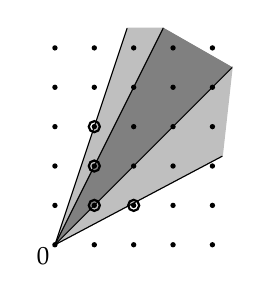
\begin{tikzpicture}[scale=0.5]
	\filldraw[lightgray] (0,0) -- (1.833,5.5) -- (2.75,5.5)  -- cycle;
	\filldraw[gray] (0,0)  -- (2.75,5.5) -- (4.5,4.5)  -- cycle;
	\filldraw[lightgray] (0,0)  -- (4.25,2.25) -- (4.5,4.5)  -- cycle;
	\draw (0,0) -- (1.833,5.5);
	\draw (0,0) -- (2.75,5.5);
	\draw (0,0) -- (4.5,4.5);
	\draw (0,0) -- (4.25,2.25) node at (-0.3,-0.3){\small $0$};
	\foreach \x in {0,...,4}
	\foreach \y in {0,...,5}
	{
		\filldraw[fill=black] (\x,\y)  circle (1.5pt);
	}
	\draw[black,thick] (1,1) circle (4pt);
	\draw[black,thick] (1,2) circle (4pt);
	\draw[black,thick] (1,3) circle (4pt);
	\draw[black,thick] (2,1) circle (4pt);
	\end{tikzpicture}	
\end{wrapfigure}

As an example for the usefulness of PyNormaliz we write a small function
that creates the intersection of two cones - something which would be
quite messy if we work with input files.

    \begin{Verbatim}[commandchars=\\\{\}]
{\color{incolor}In [{\color{incolor}9}]:} \PY{k}{def} \PY{n+nf}{intersection}\PY{p}{(}\PY{n}{cone1}\PY{p}{,} \PY{n}{cone2}\PY{p}{)}\PY{p}{:}
            \PY{n}{intersection\PYZus{}ineq} \PY{o}{=} \PY{n}{cone1}\PY{o}{.}\PY{n}{SupportHyperplanes}\PY{p}{(}\PY{p}{)}\PY{o}{+}\PY{n}{cone2}\PY{o}{.}\PY{n}{SupportHyperplanes}\PY{p}{(}\PY{p}{)}
            \PY{n}{C} \PY{o}{=} \PY{n}{Cone}\PY{p}{(}\PY{n}{inequalities} \PY{o}{=} \PY{n}{intersection\PYZus{}ineq}\PY{p}{)}
            \PY{k}{return} \PY{n}{C}
        
        \PY{n}{C1} \PY{o}{=} \PY{n}{Cone}\PY{p}{(}\PY{n}{cone}\PY{o}{=}\PY{p}{[}\PY{p}{[}\PY{l+m+mi}{1}\PY{p}{,}\PY{l+m+mi}{2}\PY{p}{]}\PY{p}{,}\PY{p}{[}\PY{l+m+mi}{2}\PY{p}{,}\PY{l+m+mi}{1}\PY{p}{]}\PY{p}{]}\PY{p}{)}
        \PY{n}{C2} \PY{o}{=} \PY{n}{Cone}\PY{p}{(}\PY{n}{cone}\PY{o}{=}\PY{p}{[}\PY{p}{[}\PY{l+m+mi}{1}\PY{p}{,}\PY{l+m+mi}{1}\PY{p}{]}\PY{p}{,}\PY{p}{[}\PY{l+m+mi}{1}\PY{p}{,}\PY{l+m+mi}{3}\PY{p}{]}\PY{p}{]}\PY{p}{)}
        \PY{n+nb}{print}\PY{p}{(}\PY{n}{intersection}\PY{p}{(}\PY{n}{C1}\PY{p}{,}\PY{n}{C2}\PY{p}{)}\PY{o}{.}\PY{n}{ExtremeRays}\PY{p}{(}\PY{p}{)}\PY{p}{)}
\end{Verbatim}

    \begin{Verbatim}[commandchars=\\\{\}]
[[1, 1], [1, 2]]

    \end{Verbatim}

%    \begin{Verbatim}[commandchars=\\\{\}]
%{\color{incolor}In [{\color{incolor}10}]:} \PY{k}{def} \PY{n+nf}{magic\PYZus{}square}\PY{p}{(}\PY{n}{n}\PY{p}{)}\PY{p}{:}
%             \PY{n}{equation} \PY{o}{=} \PY{p}{[}\PY{l+m+mi}{1} \PY{k}{if} \PY{n}{x}\PY{o}{\PYZlt{}}\PY{n}{n} \PY{k}{else} \PY{l+m+mi}{0} \PY{k}{for} \PY{n}{x} \PY{o+ow}{in} \PY{n+nb}{range}\PY{p}{(}\PY{n}{n}\PY{o}{*}\PY{o}{*}\PY{l+m+mi}{2}\PY{p}{)}\PY{p}{]}
%             \PY{n}{eqs} \PY{o}{=} \PY{p}{[}\PY{p}{]}
%         
%             \PY{k}{for} \PY{n}{i} \PY{o+ow}{in} \PY{n+nb}{range}\PY{p}{(}\PY{l+m+mi}{1}\PY{p}{,}\PY{n}{n}\PY{p}{)}\PY{p}{:}
%                 \PY{n}{equation} \PY{o}{=} \PY{p}{[}\PY{l+m+mi}{1} \PY{k}{if} \PY{n}{x}\PY{o}{\PYZlt{}}\PY{n}{n} \PY{k}{else} \PY{l+m+mi}{0} \PY{k}{for} \PY{n}{x} \PY{o+ow}{in} \PY{n+nb}{range}\PY{p}{(}\PY{n}{n}\PY{o}{*}\PY{o}{*}\PY{l+m+mi}{2}\PY{p}{)}\PY{p}{]}
%                 \PY{k}{for} \PY{n}{j} \PY{o+ow}{in} \PY{n+nb}{range}\PY{p}{(}\PY{n}{n}\PY{p}{)}\PY{p}{:}
%                     \PY{n}{equation}\PY{p}{[}\PY{n}{i} \PY{o}{*} \PY{n}{n} \PY{o}{+} \PY{n}{j}\PY{p}{]} \PY{o}{=} \PY{o}{\PYZhy{}}\PY{l+m+mi}{1}
%                 \PY{n}{eqs}\PY{o}{.}\PY{n}{append}\PY{p}{(}\PY{n}{equation}\PY{p}{)}
%         
%             \PY{k}{for} \PY{n}{i} \PY{o+ow}{in} \PY{n+nb}{range}\PY{p}{(}\PY{n}{n}\PY{p}{)}\PY{p}{:}
%                 \PY{n}{equation} \PY{o}{=} \PY{p}{[}\PY{l+m+mi}{1} \PY{k}{if} \PY{n}{x}\PY{o}{\PYZlt{}}\PY{n}{n} \PY{k}{else} \PY{l+m+mi}{0} \PY{k}{for} \PY{n}{x} \PY{o+ow}{in} \PY{n+nb}{range}\PY{p}{(}\PY{n}{n}\PY{o}{*}\PY{o}{*}\PY{l+m+mi}{2}\PY{p}{)}\PY{p}{]}
%                 \PY{n}{equation}\PY{p}{[}\PY{n}{i}\PY{p}{]} \PY{o}{=} \PY{l+m+mi}{0}
%                 \PY{k}{for} \PY{n}{j} \PY{o+ow}{in} \PY{n+nb}{range}\PY{p}{(}\PY{l+m+mi}{1}\PY{p}{,}\PY{n}{n}\PY{p}{)}\PY{p}{:}
%                     \PY{n}{equation}\PY{p}{[}\PY{n}{n}\PY{o}{*}\PY{n}{j} \PY{o}{+} \PY{n}{i}\PY{p}{]} \PY{o}{=} \PY{o}{\PYZhy{}}\PY{l+m+mi}{1}
%                 \PY{n}{eqs}\PY{o}{.}\PY{n}{append}\PY{p}{(}\PY{n}{equation}\PY{p}{)}
%         
%             \PY{n}{equation} \PY{o}{=} \PY{p}{[}\PY{l+m+mi}{1} \PY{k}{if} \PY{n}{x}\PY{o}{\PYZlt{}}\PY{n}{n} \PY{k}{else} \PY{l+m+mi}{0} \PY{k}{for} \PY{n}{x} \PY{o+ow}{in} \PY{n+nb}{range}\PY{p}{(}\PY{n}{n}\PY{o}{*}\PY{o}{*}\PY{l+m+mi}{2}\PY{p}{)}\PY{p}{]}
%             \PY{n}{diagonal} \PY{o}{=} \PY{n+nb}{list}\PY{p}{(}\PY{n}{equation}\PY{p}{)}
%             \PY{n}{anti\PYZus{}diagonal} \PY{o}{=} \PY{n+nb}{list}\PY{p}{(}\PY{n}{equation}\PY{p}{)}
%             \PY{n}{diagonal}\PY{p}{[}\PY{l+m+mi}{0}\PY{p}{]} \PY{o}{=} \PY{l+m+mi}{0}
%             \PY{n}{anti\PYZus{}diagonal}\PY{p}{[}\PY{n}{n}\PY{o}{\PYZhy{}}\PY{l+m+mi}{1}\PY{p}{]}\PY{o}{=}\PY{l+m+mi}{0}
%         
%             \PY{k}{for} \PY{n}{i} \PY{o+ow}{in} \PY{n+nb}{range}\PY{p}{(}\PY{l+m+mi}{1}\PY{p}{,} \PY{n}{n}\PY{p}{)}\PY{p}{:}
%                 \PY{n}{diagonal}\PY{p}{[}\PY{n}{n}\PY{o}{*}\PY{n}{i}\PY{o}{+}\PY{n}{i}\PY{p}{]} \PY{o}{=} \PY{o}{\PYZhy{}}\PY{l+m+mi}{1}
%                 \PY{n}{anti\PYZus{}diagonal}\PY{p}{[}\PY{n}{n}\PY{o}{*}\PY{p}{(}\PY{n}{i}\PY{o}{+}\PY{l+m+mi}{1}\PY{p}{)}\PY{o}{\PYZhy{}}\PY{p}{(}\PY{n}{i}\PY{o}{+}\PY{l+m+mi}{1}\PY{p}{)}\PY{p}{]} \PY{o}{=} \PY{o}{\PYZhy{}}\PY{l+m+mi}{1}
%             \PY{n}{eqs}\PY{o}{.}\PY{n}{append}\PY{p}{(}\PY{n}{diagonal}\PY{p}{)}
%             \PY{n}{eqs}\PY{o}{.}\PY{n}{append}\PY{p}{(}\PY{n}{anti\PYZus{}diagonal}\PY{p}{)}
%             \PY{k}{return} \PY{n}{eqs}
%         
%         \PY{n}{eqs} \PY{o}{=} \PY{n}{magic\PYZus{}square}\PY{p}{(}\PY{l+m+mi}{3}\PY{p}{)}
%         
%         \PY{k}{for} \PY{n}{line} \PY{o+ow}{in} \PY{n}{eqs}\PY{p}{:}
%             \PY{n+nb}{print}\PY{p}{(}\PY{n}{line}\PY{p}{)}
%\end{Verbatim}
%
%    \begin{Verbatim}[commandchars=\\\{\}]
%[1, 1, 1, -1, -1, -1, 0, 0, 0]
%[1, 1, 1, 0, 0, 0, -1, -1, -1]
%[0, 1, 1, -1, 0, 0, -1, 0, 0]
%[1, 0, 1, 0, -1, 0, 0, -1, 0]
%[1, 1, 0, 0, 0, -1, 0, 0, -1]
%[0, 1, 1, 0, -1, 0, 0, 0, -1]
%[1, 1, 0, 0, -1, 0, -1, 0, 0]
%
%    \end{Verbatim}

    A magic square is an \(n\times n\) table in which each row and column
and the two diagonals sum up to the same magic constant \(\mathcal{M}\).
The function
\begin{Verbatim}
magic_square(n)
\end{Verbatim}
generates all defining equations of the \(n\times n\) magic squares.

So only a few lines of code are necessary to create the respective cone
and compute its Hilbert basis (in the dual mode) and Hilbert series.

    \begin{Verbatim}[commandchars=\\\{\}]
{\color{incolor}In [{\color{incolor}11}]:} \PY{n}{n}\PY{o}{=}\PY{l+m+mi}{4}
         \PY{n}{grading} \PY{o}{=} \PY{p}{[}\PY{l+m+mi}{1} \PY{k}{if} \PY{n}{x}\PY{o}{\PYZlt{}}\PY{n}{n} \PY{k}{else} \PY{l+m+mi}{0} \PY{k}{for} \PY{n}{x} \PY{o+ow}{in} \PY{n+nb}{range}\PY{p}{(}\PY{n}{n}\PY{o}{*}\PY{o}{*}\PY{l+m+mi}{2}\PY{p}{)}\PY{p}{]}
         \PY{n}{M} \PY{o}{=} \PY{n}{Cone}\PY{p}{(}\PY{n}{equations}\PY{o}{=}\PY{n}{magic\PYZus{}square}\PY{p}{(}\PY{n}{n}\PY{p}{)}\PY{p}{,}\PY{n}{grading}\PY{o}{=}\PY{n}{grading}\PY{p}{)}
         \PY{n+nb}{print}\PY{p}{(}\PY{n+nb}{len}\PY{p}{(}\PY{n}{M}\PY{o}{.}\PY{n}{HilbertBasis}\PY{p}{(}\PY{n}{DualMode}\PY{o}{=}\PY{k+kc}{True}\PY{p}{)}\PY{p}{)}\PY{p}{)}
         \PY{n+nb}{print}\PY{p}{(}\PY{n}{M}\PY{o}{.}\PY{n}{HilbertSeries}\PY{p}{(}\PY{p}{)}\PY{p}{)}
\end{Verbatim}

    \begin{Verbatim}[commandchars=\\\{\}]
20
[[1, 4, 18, 36, 50, 36, 18, 4, 1], [1, 1, 1, 1, 2, 2, 2, 2], 0]

    \end{Verbatim}   
    \end{document}
